\documentclass[letterpaper,12pt]{article}

% IMPORT PACKAGES
\usepackage{amsmath, amsfonts, amssymb, amsthm}		% math equations
\usepackage{commath}								% more math equations
\usepackage{ifthen}									% conditional statements
\usepackage{pgfplots}
\usepackage{calc}  
\usepackage{tikz}
\usepackage{fancyhdr}
\usepackage[shortlabels]{enumitem}					% use letters to enumerate
\usepackage[english]{babel} 						% language-based hyphenation
\usepackage{blindtext}								% example text
\usepackage{microtype}								% improve justification
\usepackage{wrapfig}								% wraps words around figures
\usepackage{enumitem}								% improve lists
\usepackage{index}									% indices
\usepackage{lastpage}
\usepackage{extramarks}
\usepackage[plain]{algorithm}
\usepackage{algpseudocode}
\usepackage{matlab-prettifier}
\usepackage{verbatim}
\usepackage{fancyvrb}
\usepackage{actuarialsymbol}
\makeindex
\pgfplotsset{width = 9.5cm}
\pgfplotsset{compat=1.5}

\usepackage{graphicx}								% use pictures
\graphicspath{ {./out/} }

\usepackage{hyperref}								% hyperlinks
\hypersetup{
    colorlinks=true,
    linkcolor=blue,
    filecolor=magenta,      
    urlcolor=cyan,
    pdfpagemode=FullScreen,
    }

\usetikzlibrary{automata,positioning}

% CHANGE PAGE MARGINS
\usepackage[letterpaper, inner=1in, outer=1in, top=1in, bottom=1in, bindingoffset=0in]{geometry}

% CHANGE FONT
\usepackage{mathpple}
\usepackage{dsfont,listings}
%\usepackage{lmodern}
%\usepackage[T1]{fontenc}
%\usepackage{mathptmx}
%\usepackage[textwidth=6.5in, textheight=9in]{geometry}

% HEADER/FOOTER
\pagestyle{fancy}
\fancyhf{}
\setlength{\headheight}{28pt}
\lhead{\Class \\ \Title}
\rhead{\AuthorName \\ \ClassInstructor}
\cfoot{\thepage\ of \pageref{LastPage} }

% TITLE PAGE
\title{
    \vspace{2in}
    \textmd{\textbf{\Class:\ \\ \Title}}\\
    \vspace{3in}
}
    \author{\AuthorName \vspace{2pt}\\ \textit{\ClassInstructor}}
	\date{}

% CUSTOM GLOBAL COMMANDS
\newcommand{\Title}{Beginning Scientific Computing}
\newcommand{\Date}{May 7th, 2023}
\newcommand{\Class}{Learning MATLAB}
\newcommand{\ClassInstructor}{Professor Tae Eun Kim}
\newcommand{\AuthorName}{Ian McCamey}

\newcommand{\alg}[1]{\textsc{\bfseries \footnotesize #1}}
\newcommand{\deriv}[1]{\frac{\mathrm{d}}{\mathrm{d}x} (#1)}
\newcommand{\pderiv}[2]{\frac{\partial}{\partial #1} (#2)}
\newcommand{\E}{\mathrm{E}}
\newcommand{\Var}{\mathrm{Var}}
\newcommand{\Cov}{\mathrm{Cov}}
\newcommand{\Bias}{\mathrm{Bias}}
\def\code#1{\texttt{#1}}

\begin{document}
\maketitle
\pagebreak

\section*{Introduction}
This report contains an overview of my work in completing MATH 3607, Beginning Scientific Computing, a course specializing in the programming and numeric computing platform MATLAB at The Ohio State University during the Spring of 2023.  The course was designed as an introduction to the mathematical theory of algorithms used to solve problems that typically arise in sciences, engineering, and finance.  Specifically, several key concepts taught in this course are applicable to the main responsibilities of actuaries, data scientists, and other quantitative thinkers. 

My purpose in presenting this document publicly is to showcase my experience in utilizing statistical software to solve complex mathematical problems via numerical computations.  In addition, given the complexity of the mathematics involved, I hope to reduce each problem into a digestible form for a non-technical reader to understand, as this kind of conceptual simiplification is necessary when communicating with others in the professional world.

It is worthy to note that the programming language R is more commonly used in the actuarial profession for data-driven calculations and analysis. However, it and MATLAB share many commonalities. In particular, both
\begin{itemize}
	\item are used for numerical computations,
	\item support functional programming,
	\item support array programming (vectorized operations),
	\item allow plotting of functions and data, and
	\item allow implementation of algorithms.
\end{itemize}

As to where they differ, an experienced programmer knows that their syntactical differences are minor compared to their conceptual similarities.  However, R admittedly has a greater ability to handle and manipulate large datasets, while MATLAB can apply the theories of linear algebra far better than R.  A near-comprehensive comparison between the two languages can be found \href{https://cran.r-project.org/doc/contrib/Hiebeler-matlabR.pdf}{here} in a PDF from the University of Maine.

Let's begin to see how MATLAB can be used to gain insight about the nature of our world through mathematical models and computation.

\pagebreak

\begin{description}

\item{\textbf{Annuities.}}	\\
A basic type of investment is an annuity: one makes monthly deposits of size $P$ for $n$ months at a fixed annual effective interest rate $i$, and at maturity collects the amount
$$ F = P \ax{\angln i} = P \left(\frac{(1+i)^n - 1}{i}\right). $$ 
Say you want to create an annuity for a term of $300$ months and final value of \$1,000,000. Using MATLAB, you can make a table of the interest rate you will need to get for each of the different contribution values $P = 500, 550, \dots , 1000$. Implementing this into code, we can write:

\begin{lstlisting}[
frame=single,
style=Matlab-editor]
n = 300;
F = 1000000;

for P = 500:50:1000
    if P == 500
        fprintf(' %10s %12s\n', 'Payment, P', 'Rate, r')
        fprintf(' %25s\n', repmat('-', 1, 25))
    end
    % function definition
    f = @(i) P*((1 + i)^n - 1)/i - S;	
    % finding roots
    i = fzero(f, [eps 1]);
    fprintf(' %10d %12.6f\n', P, i)
end
\end{lstlisting}

which prints the following to the console:
\VerbatimInput{out/out01.txt}

\pagebreak

\item{\textbf{Random Walks.}}	\\
In a computer, data is stored as a finite number of bits. Therefore, not every number can be stored \textit{exactly}; there is a small error between the number and its computer-based (floating point) representation.  It’s reasonable to expect, then, that floating point errors accumulate randomly during a long computation. 

On average we expect as many errors to be negative as positive, so they tend to partially cancel out. In fact, a classical result of probability is that, as the number of computations increases, the average of all of these random errors is very near $0$.

Here is a plot of 50 simulations of this randomly compounding error in MATLAB.

\begin{lstlisting}[
frame=single,
style=Matlab-editor]
clf
rng(6960)
n = 10000;
n_walks = 50;

for i = 1:n_walks
    % generate random errors
    r = randn(n,1); 
    % accumulate errors
    y = cumsum(sign(r));	
    plot(y(1:5:end)), hold on
end
title('50 Random Walks')
\end{lstlisting}
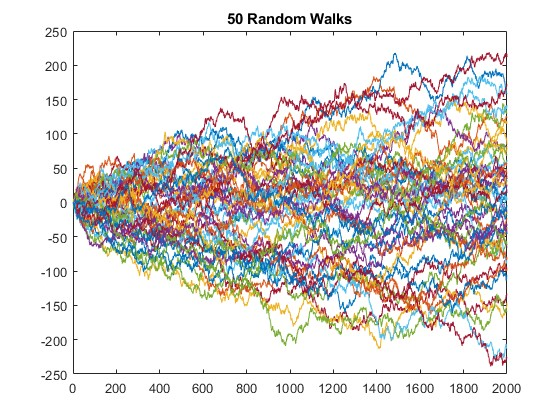
\includegraphics[scale=0.7]{random_walks}

\end{description}

\end{document}